\documentclass[11pt]{amsart}

\usepackage[utf8]{inputenc}
\usepackage{a4wide}
\usepackage{amssymb,amsmath,amsthm,newlfont,enumerate}
\usepackage{appendix}
\usepackage{dsfont}
\usepackage{amsfonts}
\usepackage{amssymb}
\usepackage{amsbsy}
\usepackage[dvips]{graphicx}
\usepackage{epstopdf}
\usepackage{psfrag}
\usepackage[hang,center]{caption}
\usepackage{verbatim} 
\usepackage{float}
\usepackage{cite}
\usepackage[colorlinks=true,linkcolor=blue,urlcolor=blue]{hyperref}
%\usepackage{hyperref}
\usepackage{color}
\usepackage[normalem]{ulem}
\usepackage{fancyhdr}
\usepackage{bm}
\usepackage{xcolor}
\usepackage{empheq}
\usepackage{placeins}
%\usepackage[all,cmtip]{xy}
\usepackage{tikz}
%\usetikzlibrary{cd}
\usetikzlibrary{positioning}
\usetikzlibrary{matrix}
\usepackage[]{showkeys}
\usepackage{nccmath}
%\usepackage{mathtools}
%\mathtoolsset{showonlyrefs}

\def\NN{\mathbb{N}}
\def\QQ{\mathbb{Q}}
\def\RR{\mathbb{R}}
\def\CC{\mathbb{C}}
\def\FF{\mathbb F}
\def\PP{\mathbb P}

\def\cA{\mathcal A}
\def\cB{\mathcal B}
\def\cC{\mathcal C}
\def\cD{\mathcal D}
\def\cE{\mathcal E}
\def\cF{\mathcal F}
\def\cG{\mathcal G}
\def\cH{\mathcal H}
\def\cO{\mathcal O}
\def\cP{\mathcal P}
\def\cR{\mathcal R}
\def\cQ{\mathcal Q}
\def\cN{\mathcal N}
\def\cX{\mathcal X}
\def\cY{\mathcal Y}
\def\cz{\mathcal z}
\def\cT{\mathcal T}
\def\cM{\mathcal M}
\def\cS{\mathcal S}
\def\cV{\mathcal V}
\def\cL{\mathcal L}
\def\cZ{\mathcal Z}
\def\cK{\mathcal K}

\def\cAij{\mathcal A_{ij}}
\def\cBij{\mathcal B_{ij}}
\def\cCij{\mathcal C_{ij}}
\def\cDij{\mathcal D_{ij}}
\def\cEij{\mathcal E_{ij}}
\def\cFij{\mathcal F_{ij}}
\def\cGij{\mathcal G_{ij}}
\def\cCij{\mathcal H_{ij}}

\newcommand{\xb}{\mathbf{x}}
\newcommand{\rb}{\mathbf{r}}
\newcommand{\vb}{\mathbf{v}}
\newcommand{\zb}{\mathbf{z}}
\newcommand{\ub}{\mathbf{u}}
\newcommand{\eb}{\mathbf{e}}
\newcommand{\jb}{\mathbf{j}}
\newcommand{\Eb}{\mathbf{E}}
\newcommand{\Bb}{\mathbf{B}}
\newcommand{\ab}{\mathbf{a}}
\newcommand{\bb}{\mathbf{b}}
\newcommand{\cb}{\mathbf{c}}
\newcommand{\mb}{\mathbf{m}}
\newcommand{\nb}{\mathbf{n}}
\newcommand{\Ab}{\mathbf{A}}
\newcommand{\db}{\mathbf{d}}
\newcommand{\kb}{\mathbf{k}}
\newcommand{\Ub}{\mathbf{U}}
\newcommand{\Jb}{\mathbf{J}}
\newcommand{\pb}{\mathbf{p}}
\newcommand{\qb}{\mathbf{q}}
\newcommand{\Mb}{\mathbf{M}}
\newcommand{\Xb}{\mathbf{X}}
\newcommand{\Vb}{\mathbf{V}}
\newcommand{\Zb}{\mathbf{Z}}
\newcommand{\Rb}{\mathbf{R}}
\newcommand{\lb}{\mathbf{\ell}}
\newcommand{\vs}{v_{\perp}}
\newcommand{\rhob}{\boldsymbol{\rho}}
\newcommand{\gamb}{\boldsymbol{\gamma}}
\newcommand{\psib}{\boldsymbol{\psi}}
\newcommand{\etab}{\boldsymbol{\eta}}
\newcommand{\xib}{\boldsymbol{\xi}}
\newcommand{\thetab}{\boldsymbol{\theta}}
\newcommand{\pab}{\boldsymbol{\partial}}
\newcommand{\omb}{\boldsymbol{\omega}}
\newcommand{\Lamb}{\boldsymbol{\Lambda}}
\newcommand{\Gamb}{\boldsymbol{\Gamma}}
\newcommand{\Xib}{\boldsymbol{\Xi}}
\newcommand{\Thetab}{\boldsymbol{\Theta}}

\let\eps\varepsilon
\let\wt\widetilde
\let\tn\textnormal
\let\vphi\varphi
\let\pa\partial
\let\para\parallel
\let\wh\widehat
\let\ttt\texttt

\newcommand{\grad}{\tn{grad}}
\newcommand{\curl}{\tn{curl}}
\renewcommand{\div}{\tn{div}}
\renewcommand{\Im}{\tn{Im}}

\def\be{\begin{equation}}
\def\ee{\end{equation}}
\def\bes{\begin{equation*}}
\def\ees{\end{equation*}}

\DeclareMathOperator{\arctantwo}{arctan2}

\newcommand{\fder}[2]{\frac{\delta #1}{\delta #2}}
\newcommand{\pder}[2]{\frac{\partial #1}{\partial #2}}
\newcommand{\intv}[1]{\int_{\RR^3} #1\,d\bfv }
\newcommand{\parfra}[2]{\frac{\partial #1}{\partial #2}}
\newcommand{\paz}[2]{\frac{\partial #1}{\partial z_{#2}}}
\newcommand{\pay}[2]{\frac{\partial #1}{\partial y_{#2}}}
\newcommand{\dt}[1]{\frac{\mathrm d #1}{\mathrm dt}}
\newcommand{\dtpr}[1]{\frac{\mathrm d #1}{\mathrm dt'}}
\newcommand{\ds}[1]{\frac{\mathrm d #1}{\mathrm ds}}
\newcommand{\dalph}[1]{\frac{d #1}{d\theta}}
\newcommand{\dlam}[1]{\frac{d #1}{d\lambda}}
\newcommand{\gavg}[1]{\langle #1 \rangle}

%\newcommand{\gavg}[1]{\overline{ #1 }}

\newcommand{\stef}[1]{\color{blue}#1 \color{black}}
\newcommand{\alert}[1]{\color{red}#1 \color{black}}
\newcommand{\delet}[1]{{\tiny \sout{#1}}}

\theoremstyle{definition}
\newtheorem{definition}{Definition}
\newtheorem{assumption}{Assumption}
\newtheorem{remark}{Remark}
\newtheorem*{example*}{Example}

\theoremstyle{plain}
\newtheorem{lemma}{Lemma}
\newtheorem{prop}{Proposition}
\newtheorem{theorem}{Theorem}
\newtheorem*{theorem*}{Theorem}
\newtheorem{corollary}[theorem]{Corollary}
\newtheorem{propT}{Proposition}
\newtheorem{thmT}{Theorem}

\title{Finite Element Exterior Calculus (FEEC)}

\begin{document}

\maketitle

\begin{abstract}
 This is a draft for a lecture I plan to give at some point. 
\end{abstract}


\section{Introduction}
%This lecture is \cite{ArnoldFalkWinther2006,ArnoldFalkWinther2010}.
%\tableofcontents

\bigskip

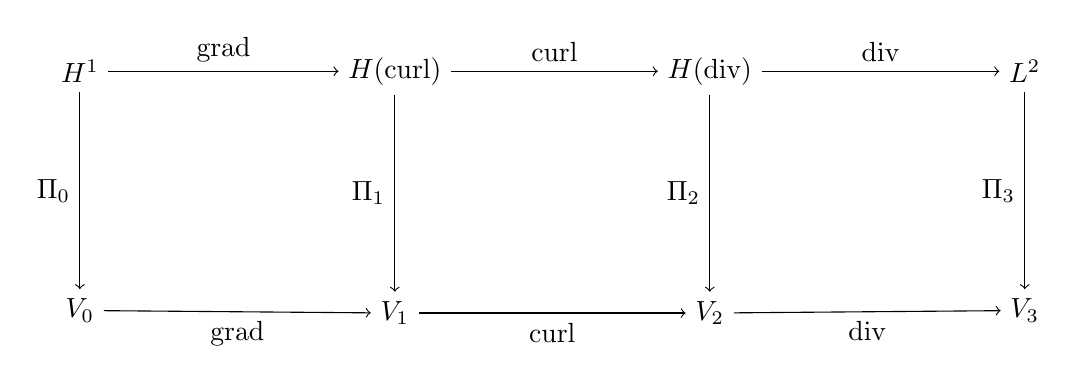
\begin{tikzpicture}[align=center, node distance=4cm, auto]
  \node (H1) {$H^1$};
  \node (V0) [below=2.5cm of H1] {$V_0$};
  \node (Hcurl) [right of=H1] {$H(\tn{curl})$};
  \node (V1) [below=2.5cm of Hcurl] {$V_1$};
  \node (Hdiv) [right of=Hcurl] {$H(\tn{div})$};
  \node (V2) [below=2.5cm of Hdiv] {$V_2$};
  \node (L2) [right of=Hdiv] {$L^2$};
  \node (V3) [below=2.5cm of L2] {$V_3$};
  \draw[->] (H1) to node {$\grad$} (Hcurl);
  \draw[->] (H1) to node [swap] {$\Pi_0$} (V0);
  \draw[->] (Hcurl) to node {$\curl$} (Hdiv);
  \draw[->] (Hcurl) to node [swap] {$\Pi_1$} (V1);
  \draw[->] (Hdiv) to node {$\div$} (L2);
  \draw[->] (Hdiv) to node [swap] {$\Pi_2$} (V2);
  \draw[->] (L2) to node [swap] {$\Pi_3$} (V3);
  \draw[->] (V0) to node [swap] {$\grad$} (V1);
  \draw[->] (V1) to node [swap] {$\curl$} (V2);
  \draw[->] (V2) to node [swap] {$\div$} (V3);
\end{tikzpicture}

\bigskip
\bigskip

\begin{tikzpicture}[align=center, node distance=4cm, auto]
  \node (H1) {$H^1_0$};
  \node (V0) [below=2.5cm of H1] {$V_0$};
  \node (L2) [right of=H1] {$L^2$};
  \node (V1) [below=2.5cm of L2] {$V_1$};
  \draw[->] (H1) to node {$\pder{}{x}$} (L2);
  \draw[->] (H1) to node [swap] {$\Pi_0$} (V0);
  \draw[->] (L2) to node [swap] {$\Pi_1$} (V1);
  \draw[->] (V0) to node [swap] {$\pder{}{x}$} (V1);
\end{tikzpicture}




\section{Old notes from MHD hybrid}

\subsection{Differential forms}
We give here some basic information about differential forms needed in the course of this work, 
with emphasis on the the case where the ambient space is a three-dimensional differentiable 
manifold 
$\cM \subset \RR^3$. A full account of the theory can be found for instance in 
\cite{Arnold,Frankel}. 

Denoting by $\ttt x \in \cM$ a point on the manifold, the tangent space at $\ttt{x}$ is 
$T_\ttt{x}\cM \equiv \RR^3$, whose elements are called ``vectors'' $\ttt v \in 
T_\ttt{x}\cM$. Let us assume for simplicity that the manifold $\cM$ can be described by a single 
coordinate chart $\vphi:U\to \cM$, $\Gamb \mapsto \ttt{x}$, where $\Gamb=(q_1,q_2,q_3)\in U\subset 
\RR^3$ are called the 
coordinates of $\ttt{x}$ under the chart $\vphi$. Then a basis of $T_\ttt{x} \cM$ is given by 
the columns of the Jacobian $D\vphi = (\pa\vphi_i/\pa q_j)_{i,j}$, which we denote by $\pab_j := 
(\pa\vphi_i/q_j)_i$. The components of a vector $\ttt v \in T_\ttt{x}\cM$ in this basis are 
denoted by $\vb = (v^1,v^2,v^3)$, hence
\be \label{geom:v}
 \ttt v = \sum_j v^j\,\pab_j = (D\vphi) \vb\,.
\ee
The dual of the tangent space at $\ttt x$ is the cotangent space $T^*_\ttt{x}\cM$, whose 
elements are linear forms on $T_\ttt{x}\cM$, i.e. for $\ttt p \in 
T^*_\ttt{x}\cM$ one has $\ttt p: T_\ttt{x}\cM \to \RR$. It is easy to see that a dual 
basis is given by the lines of $D\vphi^{-1}$; we denote this basis by 
d$q^j:=(\pa\vphi^{-1}_j/\pa x_i)$. The components of a ``covector'' $\ttt p \in 
T_\ttt{x}^*\cM$ in this basis are denoted by $\pb = (p_1,p_2,p_3)$, hence
\be \label{geom:p}
 \ttt p = \sum_j p_j\,\tn d q^j = (D\vphi)^{-\top} \pb\,.
\ee
The notation in \eqref{geom:v} and \eqref{geom:p} deserves a few remarks: $\ttt v$ and $\ttt 
p$ are geometrical objects, whereas $\vb$ and $\pb$ denote the representation of these objects in 
the bases induced by the coordinate chart $\vphi$. Moreover, the coordinates of vectors are written 
with an upper index, whereas the coordinates of covectors carry a lower index. The action of a 
covector $\ttt p$ on a vector $\ttt v$ is then conveniently written as 
\be \label{p(v)}
\ttt p(\ttt v) = p_j v^j = \pb \cdot \vb\,,
\ee
where the sum convention is implied for repeated indices. As a direct consequence of \eqref{p(v)} 
we 
have
\be
 \tn dq^j(\ttt v) = v^j\,.
\ee

\begin{definition}
 ({\bf $p$-forms}.) A $p$-form $\omega^p$ is a $p$-linear form on $T_\ttt{x}\cM \times \ldots 
\times 
T_\ttt{x}\cM$ ($p$ times), which is alternating, i.e.
$$
 \omega^p: T_\ttt{x}\cM \times \ldots \times T_\ttt{x}\cM \to \RR\,,\qquad\quad 
(\ttt{v}_1,\ldots,\ttt{v}_p) 
\mapsto \omega^p(\ttt{v}_1,\ldots,\ttt{v}_p)\,,
$$
such that
$$
 \omega^p(\ldots,\ttt{v}_i,\ldots,\ttt{v}_j,\ldots) = - 
\omega^p(\ldots,\ttt{v}_j,\ldots,\ttt{v}_i,\ldots)\,.
$$
\end{definition}

Due to the above definition, covectors $\ttt p \in T_\ttt{x}^*\cM$ can be identified with $1$-forms 
$\omega^1$. Using the basis introduced in \eqref{geom:p}, in the three-dimensional case we write
\be
 \omega^1_\pb := p_1\,\tn d q^1 + p_2\,\tn d q^2 + p_3\,\tn d q^3\,.
\ee
The tensor product of two $1$-forms is defined as
\be
 \omega^1_\ab \otimes \omega^1_\bb(\ttt v, \ttt w) := \omega^1_\ab(\ttt v)\,\omega^1_\bb(\ttt w)\,.
\ee
For basis vectors in particular this yields
\be
 \tn dq^i \otimes \tn dq^j(\ttt v, \ttt w) = \tn dq^i(\ttt v)\,\tn d q^j(\ttt w) = v^i w^j\,.
\ee
From the tensor product one can construct $2$-forms via the ``exterior 
product'' of two $1$-forms, defined as
\be \label{def:wedge}
 \omega^1_\ab \wedge \omega^1_\bb := \omega^1_\ab \otimes \omega^1_\bb - \omega^1_\bb \otimes 
\omega^1_\ab\,.
\ee
Clearly this object is an alternating $2$-form. For basis vectors in particular one has
\be \label{wedge:basic}
 \tn dq^i \wedge \tn dq^j(\ttt v, \ttt w) = 
  \begin{vmatrix}
    \tn dq^i(\ttt v) & \tn dq^i(\ttt w) \\ \tn dq^j(\ttt v) & \tn dq^j(\ttt w)
  \end{vmatrix}= v^i w^j - v^j w^i 
 \,,\qquad\quad \tn dq^i \wedge \tn dq^i = 0\,.
\ee
It follows that any two-form can be written as
\be
 \omega^2_\mathbf{a} := a_1\,\tn d q^2 \wedge \tn dq^3 +  a_2\,\tn d q^3 \wedge \tn dq^1 +  
a_3\,\tn d q^1 \wedge \tn dq^2 \,.
\ee
It is now easy to see that
\be
 \omega^2_{\ab \times \bb} = \omega^1_\ab \wedge \omega^1_\bb\,.
\ee
More generally, the exterior product can be defined between a $k$-form and an $l$-form so to yield 
a $k+l$-form, the mapping being antisymmetric, associative and distributive. It follows that any 
$3$-form can be written as
\be
 \omega^3_f := f\,\tn dq^1 \wedge \tn d q^2 \wedge \tn d q^3\,,
\ee
where
\be \label{det3}
 \tn dq^1 \wedge \tn d q^2 \wedge \tn d q^3(\ttt u,\ttt v, \ttt w) 
 = \begin{vmatrix}
    \tn dq^1(\ttt u) & \tn dq^1(\ttt v) & \tn dq^1(\ttt w)
    \\
    \tn dq^2(\ttt u) & \tn dq^2(\ttt v) & \tn dq^2(\ttt w)
    \\
    \tn dq^3(\ttt u) & \tn dq^3(\ttt v) & \tn dq^3(\ttt w)
   \end{vmatrix}
 = \begin{vmatrix}
    u^1 & v^1 & w^1 \\ u^2 & v^2 & w^2 \\ u^3 & v^3 & w^3
   \end{vmatrix}\,.
\ee
As a consequence of the alternating property of $p$-forms, in a manifold of dimension $n$ all 
$p$-forms with $p>n$ vanish. Therefore, to complete the picture for the case $n=3$, it remains to 
introduce the $0$-forms,
\be
 \omega^0_f = f\,,
\ee
which correspond to scalar functions. We shall denote the space of $p$-forms on the manifold $\cM$ 
by $\Lambda^p(\cM)$, $p=0,1,2,3$.

\begin{definition}
 ({\bf Interior product}.) The interior product of a $p$-form $\omega^p$ and a vector ${\ttt v \in 
T_\ttt{x}\cM}$ is the $(p-1)$-form $\tn i_\ttt{v} \omega^p$ such that
\be
 \tn i_\ttt{v} \omega^p(\ttt v_1, \ldots, \ttt v_{p-1}) := \omega^p(\ttt v, \ttt v_1,\ldots, \ttt 
v_{p-1})\,.
\ee
One denotes $\tn i_\ttt{v} \equiv \tn i_\vb$ if the choice of basis in the tangent space is clear.
\end{definition}

\noindent
For $1$-forms we obtain
\be
 \tn i_\vb \omega^1_\ab = \omega^1_\ab(\ttt v) = \ab \cdot \vb = \omega^0_{\ab \cdot \vb}\,.
\ee
For $2$-forms we use \eqref{wedge:basic} to compute
\be 
\begin{aligned}
 \tn i_\vb \omega^2_\ab(\ttt w) &= \omega^2_\ab(\ttt v, \ttt w)
 \\[2mm]
 &= a_1\,\tn d q^2 \wedge \tn dq^3(\ttt v, \ttt w) +  a_2\,\tn d q^3 \wedge \tn dq^1(\ttt v, \ttt 
w) 
 + a_3\,\tn d q^1 \wedge \tn dq^2(\ttt v, \ttt w) 
 \\[2mm]
 &= a_1 \big[ v_2 \,\tn dq^3(\ttt w) - v_3\,\tn d q^2(\ttt w) \big] + a_2 \big[ v_3 \,\tn dq^1(\ttt 
w) - v_1\,\tn d q^3(\ttt w) \big] + a_3 \big[ v_1 \,\tn dq^2(\ttt w) - v_2\,\tn d q^1(\ttt w) \big]
 \\[2mm]
 &= (a_2 v_3 - a_3 v_2)\, \tn d q^1(\ttt w) + (a_3 v_1 - a_1 v_3)\, \tn d q^2(\ttt w) + (a_1 v_2 - 
a_2 v_1)\, \tn d q^3(\ttt w)\,.
\end{aligned}
\ee
Thus $\tn i_\vb \omega^2_\ab = \omega^1_{\ab \times \vb}$. For $3$-forms, from \eqref{det3} 
one obtains
\be
\begin{aligned}
 \tn i_\ub \omega^3_f (\ttt v, \ttt w) &= \omega^3_f(\ttt u, \ttt v, \ttt w)
 \\[2mm]
 &= f\,\tn dq^1 \wedge \tn d q^2 \wedge \tn d q^3(\ttt u, \ttt v, \ttt w)
 \\[2mm]
 &= f\, \begin{vmatrix}
    \tn dq^1(\ttt u) & \tn dq^1(\ttt v) & \tn dq^1(\ttt w)
    \\
    \tn dq^2(\ttt u) & \tn dq^2(\ttt v) & \tn dq^2(\ttt w)
    \\
    \tn dq^3(\ttt u) & \tn dq^3(\ttt v) & \tn dq^3(\ttt w)
   \end{vmatrix}
 \\[2mm]
 &= f\, u_1 \big[\tn d q^2(\ttt v)\,\tn d q^3(\ttt w) - \tn d q^3(\ttt v)\,\tn d q^2(\ttt w) \big] 
- f\, u_2 \big[\tn d q^1(\ttt v)\,\tn d q^3(\ttt w) - \tn d q^3(\ttt v)\,\tn d q^1(\ttt w) \big]
 \\[2mm]
 &\qquad + f\, u_3 \big[\tn d q^1(\ttt v)\,\tn d q^2(\ttt w) - \tn d q^2(\ttt v)\,\tn d q^1(\ttt w) 
\big]
 \\[2mm]
 &= f\,u_1\,\tn d q^2 \wedge \tn d q^3(\ttt v,\ttt w) + f\,u_2\,\tn d q^3 \wedge \tn d q^1(\ttt 
v,\ttt w) + f\,u_3\,\tn d q^1 \wedge \tn d q^2(\ttt v,\ttt w)\,.
\end{aligned}
\ee
Thus $\tn i_\ub \omega^3_f = \omega^2_{f\ub}$.


\begin{definition}
 ({\bf Exterior derivative}.) The exterior derivative is the unique operator\\ ${\tn 
d:\Lambda^p(\cM) \to \Lambda^{p+1}(\cM)}$ satisfying:
 \begin{enumerate}[(i)]
  \item $\tn d (\omega^p_\ab + \omega^p_\bb ) = \tn d \omega^p_\ab + \tn d \omega^p_\bb$,
  \item $\tn d \omega^0_f \equiv \tn d f = \omega^1_{\grad f}$ is the usual differential of a 
function $f$,
  \item Leibniz rule: $\tn d(\omega^p \wedge \omega^q) = \tn d \omega^p \wedge \omega^q + (-1)^p\, 
\omega^p \wedge \tn d \omega^q$,
  \item $\tn d^2 \omega^p = \tn d (\tn d \omega^p) = 0\,.$
 \end{enumerate}
\end{definition}

\noindent
For zero forms ($p=0$) the Leibniz rule yields
\be
\begin{aligned}
  \tn d(f\,\omega^q) = \tn d(\omega^0_f \wedge \omega^q) &= \tn d \omega^0_f \wedge \omega^q + 
\omega^0_f \wedge \tn d \omega^q
 \\[2mm]
 &= \omega^1_{\grad f} \wedge \omega^q + f\, \tn d \omega^q\,.
\end{aligned}
\ee
This can be used to compute the exterior derivative of a $1$-form,
\be
\begin{aligned}
 \tn d \omega^1_\ab &= \tn d (a_1\,\tn d q^1) + \tn d (a_2\,\tn d q^2) + \tn d (a_3\,\tn d q^3)
 \\[2mm]
 &= \omega^1_{\grad\,a_1} \wedge \tn d q^1 + \omega^1_{\grad\,a_2} \wedge \tn d q^2  + 
\omega^1_{\grad\,a_3} \wedge \tn d q^3
 \\[2mm]
 &= \left( \parfra{a_3}{q^2} - \parfra{a_2}{q^3} \right)\,\tn d q^2 \wedge \tn dq^3 +  \left( 
\parfra{a_1}{q^3} - \parfra{a_3}{q^1} \right)\,\tn d q^3 
\wedge \tn dq^1 + \left( \parfra{a_2}{q^1} - \parfra{a_1}{q^2} \right)\,\tn d q^1 \wedge \tn dq^2
 \\[2mm]
 &= \omega^2_{\curl\,\ab} \,.
\end{aligned}
\ee
For a $2$-form one obtains
\be
\begin{aligned}
 \tn d \omega^2_\ab &= \tn d (a_1\,\tn d q^2 \wedge \tn dq^3) + \tn d ( a_2\,\tn d q^3 
\wedge \tn dq^1) + \tn d( a_3\,\tn d q^1 \wedge \tn dq^2)
 \\[2mm]
 &= \omega^1_{\grad\,a_1} \wedge \tn d q^2 \wedge \tn dq^3 + \omega^1_{\grad\,a_2} \wedge \tn d q^3 
\wedge \tn dq^1 + \omega^1_{\grad\,a_3} \wedge \tn d q^1 \wedge \tn dq^2
 \\[2mm]
 &= \left( \parfra{a_1}{q^1} + \parfra{a_2}{q^2} + \parfra{a_3}{q^3} \right)\, \tn d q^1 \wedge \tn 
d q^2 \wedge \tn dq^3
 \\[2mm]
 &= \omega^3_{\div\,\ab}\,.
\end{aligned}
\ee
Finally, for a $3$-form $\omega^3\in \Lambda^3(\cM)$ we have $\tn d \omega^3 = 0$.

\begin{table}[htb]
 \caption{Summary of differential forms in $\RR^3$.} \label{tab:forms}
 \begin{tabular}{|ll|l|l|}
  \hline
  & Expression in basis & Interior product & Exterior derivative \\ 
  & & & \\
 $0$-form: & $\omega^0_f = f$ & $\tn i_\vb \omega^0_f = 0$ &  $\tn d \omega^0_f = 
\omega^1_{\grad f}$\\
 & & & \\
 $1$-form: & $\omega^1_\ab = a_1\,\tn d q^1 + a_2\,\tn d q^2 + a_3\,\tn d q^3$ & $\tn i_\vb 
\omega^1_\ab = \omega^0_{\ab \cdot \vb}$ & $\tn d \omega^1_\ab = \omega^2_{\curl\,\ab} $ \\
 & & & \\
 $2$-form: & $\omega^2_\ab := a_1\,\tn d q^2 \wedge \tn dq^3 +  a_2\,\tn d q^3 
\wedge \tn dq^1 + a_3\,\tn d q^1 \wedge \tn dq^2$ & $\tn i_\vb \omega^2_\ab = \omega^1_{\ab 
\times \vb}$ & $\tn d \omega^2_\ab = \omega^3_{\div\,\ab}$ \\
 & & & \\
 $3$-form: & $\omega^3_f = f\,\tn dq^1 \wedge \tn d q^2 \wedge \tn d q^3$ & $\tn i_\vb 
\omega^3_f = \omega^2_{f\vb}$ & $\tn d \omega^3_f = 0$\\
  \hline
 \end{tabular}
\end{table}


\subsection{The de Rham complex}

\subsection{MHD equations with FEEC}
In order to apply the FEEC framework to MHD one needs 
to identify the geometric meaning of the variables $\rho$, $\Ub$ and $\Bb$. For convenience, we set 
$k_\tn{B} = 1$ and $q_h=1$ in the following and consider the equations
\begin{subequations} \label{sys:MHD}
\begin{align}
&\pa_t \rho + \nabla \cdot (\rho \Ub) = 0\,, \label{eq:rho2}
 \\[2mm]
 &\rho ( \pa_t \Ub + \Ub \cdot \nabla \Ub) + T_0\,\nabla \rho = ( 
n_h \Ub - 
\Jb_h) \times \Bb +
\frac{1}{\mu_0}(\nabla \times \Bb) \times \Bb \,,  \label{eq:U2}
 \\[2mm]
 & \pa_t \Bb = \nabla \times (\Ub \times \Bb)\,.  \label{eq:B2}
\end{align}
\end{subequations}
From \eqref{eq:rho2} we deduce that $\rho \in \Im(\div)$ and hence $\rho$ is a 3-form,
$$
\rho \in H\Lambda^3(\Omega) \equiv L^2(\Omega)\,,\qquad \rho \equiv \rho^3 \equiv \omega^3_\rho\,.
$$
Moreover, $\rho\Ub$ is a 2-form and, according to Table \ref{tab:forms}, can be written as the 
interior product $\omega^2_{\rho \Ub} = \tn i_\Ub \omega^3_\rho$.
Similarly, from equation \eqref{eq:B2} we conclude that $\Bb \in \Im(\curl)$, thus $\Bb$ is a 
2-form,
$$
 \Bb \in H \Lambda^2(\Omega) \equiv H(\div,\Omega)\,,\qquad \Bb \equiv \Bb^2 \equiv \omega^2_\Bb\,,
$$
and that $\Ub \times \Bb$ is a 1-form, written as $\omega^1_{\Ub \times \Bb} = \tn i_{(-\Ub)} 
\omega^2_\Bb$. In the momentum equation \eqref{eq:U2} appear the terms $\nabla \rho$ and $\nabla 
\times \Bb$, which do not belong to any space of the de Rham complex. A weak formulation of this 
equation is thus necessary in order to respect the geometrical properties. Let us therefore 
multiply with a test function $\Gamb$, integrate over $\Omega$ and perform 
integration by parts in the aforementioned terms to obtain
\begin{align}
 &\int_\Omega \rho\, \pa_t \Ub \cdot \Gamb\,\tn d^3\xb + \int_\Omega \rho\Ub \cdot \nabla \Ub \cdot 
\Gamb\, \tn d^3\xb - T_0 \int_\Omega \rho\,\nabla \cdot \Gamb\, \tn d^3 \xb + 
k_\tn{B}T_0 \int_{\pa \Omega} \rho\,\Gamb \cdot \nb\,\tn d^3\xb   \label{U:weak}
 \\[2mm]
 &\: = \int_\Omega (n_h \Ub - \Jb_h) \times \Bb \cdot \Gamb\, \tn d^3\xb + 
\frac{1}{\mu_0} \int_\Omega  \Bb \cdot \nabla \times (\Bb \times \Gamb)\, \tn d^3 \xb + 
\frac{1}{\mu_0} \int_{\pa\Omega} (\nb \times \Bb) \cdot (\Bb \times \Gamb)\, \tn d^3\xb \,,  
\nonumber
\end{align}
where $\nb$ denotes the outward normal of $\Omega$ at each $\xb$. Choosing $\Gamb \in 
H\Lambda^2(\Omega)$ leads to ${\nabla \cdot \Gamb \in H\Lambda^3(\Omega)}$ being a 3-form, such 
that the $\nabla \rho$-term is now well-defined. We conclude that $\Ub$ must be a 2-form,
$$
  \Ub \in H \Lambda^2(\Omega) \equiv H(\div,\Omega)\,,\qquad \Ub \equiv \Ub^2 \equiv \omega^2_\Ub\,.
$$
Let us now check each term in \eqref{U:weak} for its geometrical properties: in the first term we 
use the interior product to write $\omega^2_{\rho\Gamb} = \tn i_{\Gamb} \omega^3_{\rho}$ such that 
two 
2-forms appear under the integral. 
From the second integration by parts we deduce 
that $\Bb\times \Gamb$ should be a 1-form, which is the case for the interior product $\tn 
i_{\Gamb} \omega^2_\Bb = \omega^1_{\Bb \times \Gamb}$. 
{\bf Boundary conditions:} ideally we want the boundary terms in \eqref{U:weak} to vanish. Hence we 
impose 
\be \label{bcs}
 \Ub \cdot \nb = 0\quad \tn {on}\,\pa\Omega\,,\qquad\quad \Bb \cdot \nb = 0 \quad 
\tn{on}\,\pa\Omega\,.
\ee
Indeed, since $(\nb \times \Bb) \cdot (\Bb \times \Gamb) = (\Bb \cdot \Gamb)(\Bb \cdot \nb) - 
|\Bb|^2 (\Gamb \cdot \nb)$ both boundary terms vanish under these conditions. We denote the 
corresponding function space by
$$
 H_0(\div,\Omega) := \{ \Gamb \in H(\div,\Omega) :\,\, \Gamb \cdot \nb = 0\,\tn{on}\,\pa\Omega \}\,.
$$
A weak formulation of \eqref{sys:MHD} reads as follows: find ${(\rho,\Ub,\Bb) \in 
L^2(\Omega) \times H_0(\div,\Omega) \times H_0(\div,\Omega)}$ such that
\begin{subequations} \label{sys:MHD:weak}
\begin{align}
& \int_\Omega \pa_t \rho\,\psi\,\tn d^3 \xb + \int_\omega \nabla \cdot (\rho \Ub)\,\psi\, \tn 
d^3\xb = 0 \quad && \forall\,\psi \in L^2(\Omega)\,, \label{eq:rho2w}
 \\[2mm]
 &\int_\Omega \rho\, \pa_t \Ub \cdot \Gamb\,\tn d^3\xb + \int_\Omega \rho\Ub \cdot \nabla \Ub \cdot 
\Gamb\, \tn d^3\xb - k_\tn{B}T_0 \int_\Omega \rho\,\nabla \cdot \Gamb\, \tn d^3 \xb  
\nonumber
 \\[2mm]
 &\:\: = \int_\Omega (q_h n_h \Ub - \Jb_h) \times \Bb \cdot \Gamb\, \tn d^3\xb + 
\frac{1}{\mu_0} \int_\Omega  \Bb \cdot \nabla \times (\Bb \times \Gamb)\, \tn d^3 \xb \quad && 
\forall\, \Gamb \in H_0(\div,\Omega)\,,  \label{eq:U2w}
 \\[2mm]
 & \int_\omega \pa_t \Bb \cdot \Thetab\, \tn d^3\xb = \int_\Omega \nabla \times (\Ub \times \Bb) 
\cdot \Thetab\,\tn d^3\xb \quad && \forall \Thetab \in H_0(\div,\Omega)\,.  \label{eq:B2w}
\end{align}
\end{subequations}



\subsection{Finite element discretization}
Let us consider the problem \eqref{sys:MHD:weak} on the finite-dimensional subspaces $V^3$ and 
$V^2_0$, which is $V^2$ with the boundary conditions \eqref{bcs}, introduced in the lower level of 
the DeRham complex in Fig. \ref{fig:derham}. Let us denote by $(\Lambda^3_i)_{i = 1\ldots N_3}$ a 
basis of $V^3 \subset L^2(\Omega)$ and by $(\Lamb^2_{i,\mu})_{i=1\ldots N_2,\mu=1,2,3}$ a basis of 
$V^2_0 \subset H_0(\div,\Omega)$, which are vector-valued functions,
$$
 \Lamb^2_{i,1} = \begin{pmatrix}
                  \Lambda^2_{i,1} \\ 0 \\ 0
                 \end{pmatrix}\,,\qquad
 \Lamb^2_{i,2} = \begin{pmatrix}
                  0 \\ \Lambda^2_{i,2} \\ 0
                 \end{pmatrix}\,,\qquad
 \Lamb^2_{i,3} = \begin{pmatrix}
                  0 \\ 0 \\ \Lambda^2_{i,3}
                 \end{pmatrix}\,.
$$
For the vector-valued basis we shall use the indexing $(\Lamb^2_I)_{I=1\ldots 3 N_2}$ with $I= 
3(i-1)+\mu$. The orthogonal projection of $\rho \in L^2(\Omega)$ on the subspace $V^3$, denoted 
by $\rho_h := \Pi_3 \rho$ is expressed in terms of the corresponding basis,
$$
 \Pi_3 \rho(\xb) = \rho_h(\xb) = \sum_{i=1}^{N_3} \rho_i\,\Lambda^3_i(\xb)\,.
$$
We define the vector $ \rhob :=(\rho_i)_{i=1\ldots N_3} \in \RR^{N_3}$ containing the coefficients 
of $\rho_h$ in the finite element basis. Similarly, for $\Ub,\Bb \in H_0(\div,\Omega)$ we have
$$
 \Pi_2 \Ub(\xb) = \Ub_h(\xb) = \sum_{I=1}^{3N_2} u_I\,\Lamb^2_I(\xb)\,,\qquad\quad \Pi_2 \Bb(\xb) = 
\Bb_h(\xb) = \sum_{I=1}^{3N_2} b_I\,\Lamb^2_I(\xb)\,,
$$
and define the vectors $\ub :=(u_I)_{I=1\ldots 3N_2}\in \RR^{3N_2}$ and $\bb :=(b_I)_{I=1\ldots 
3N_2}\in \RR^{3N_2}$. The same is done for the test functions which leads to the vectors $\psib \in 
\RR^{N_3}$, $\gamb \in \RR^{3N_2}$ and $\thetab \in \RR^{3N_2}$.



\bibliography{\string~/Desktop/PLASMA/WORK/mybib}
\bibliographystyle{ieeetr}

\end{document}